\chapter{Results}\label{chap:res}
Our system is able to produce biologically relevant dimensionality reductions that allow us to make better reduce models for \gls{cfps} systems.
We show the following key points:
\begin{itemize}
\item The reduced models produced by our system are more representative of biological data than naive models.
\item The latent space of the \gls{vae} and show that it learns a separation between the different models.
\item As noise is added to our model, the \gls{vae} performance falls off.
\item We can train a model on one dataset and predict on another dataset.
\end{itemize}

%TODO show that we're better than PCA

% Is VAE better than PCA?
% Need to use Corr-VAE in order to reconstruct space
% Noise/actually reconstructing space
% Reduction
% Biological insights
% Transfer learning

\section{Comparison of models}\label{sec:cmp}
A key goal for our system was to produce reduced models that could accurately explain our biological data.
We tested this by solving for the optimal flux distribution for each model of our reaction conditions.
We then found the correlation between the predicted output and the real biological output.
Table \ref{tab:cmp} shows the results for each of our starting models that are at the \gls{gem} scale as well as some reduced models.
As expected, we found that the full-scale \glspl{gem} have very low correlations, between $0.14$ and $0.24$.
This models are intended to describe living \ecoli cells and thus do a poor job of modeling \gls{cfps} systems.

We also compare our model to pre-existing pruned models that other algorithms have created.
For instance, the ColiPruned model from NetworkReducer has a correlation of $0.34$ with our biological data.
This is better than the full-scale genome models, though it is not as good as our customized cell-free models.
This make sense because the goal of NetworkReducer is to reduce to a minimal core model, not to specify it for cell-free systems.
Our system produces models that with more than 2x better correlations than a full-scale \gls{gem}.
While these correlations show that we still cannot perfectly describe the biological system, the reduction is far better than a full-scale model.

\begin{table}[t]
\centering
\caption{Comparison of models.
Models that have been produced by our pipeline end in 'reduced'.
We compare the full \glspl{gem} to our reduced models and show that the using our system improves the correlation with real data}
\label{tab:cmp}
\begin{tabular}{llll}
Dataset & TXTL & Correlation \\
echo    & Yes   & No        & 0.22        \\
echo    & No    & No        & 0.14        \\
hand    & Yes    & No        &   0.23     \\
hand    & No   & No        &   0.24     \\
karim   & No    & No        & 0.17      \\
coli-pruned & No & No & 0.34 \\
hand-reduced & Yes & Yes & 0.50 \\
karim-reduced & Yes & Yes & 0.43 
\end{tabular}
\end{table}

\section{Unsupervised Learning}

In addition to helping us reduce our models, we can use our trained \gls{vae} to perform unsupervised learning.
By examining the latent space, we can uncover patterns that we otherwise might not be able to discover by eye.
Figure \ref{fig:ingest} shows one way we can visualize the latent space of the \gls{vae}.
We trained our 3-layer Corr-\gls{vae} with a latent dimension of 10 on the training split of our stacked hand dataset.
We then projected the test split into then 10-dimensional latent space and passed that through the tSNE~\cite{maaten2008visualizing} to project it to 2 dimensions.
Each of the points in Figure \ref{fig:ingest} are colored according to the different starting experimental conditions.

\begin{figure}[t!]
\begin{center}
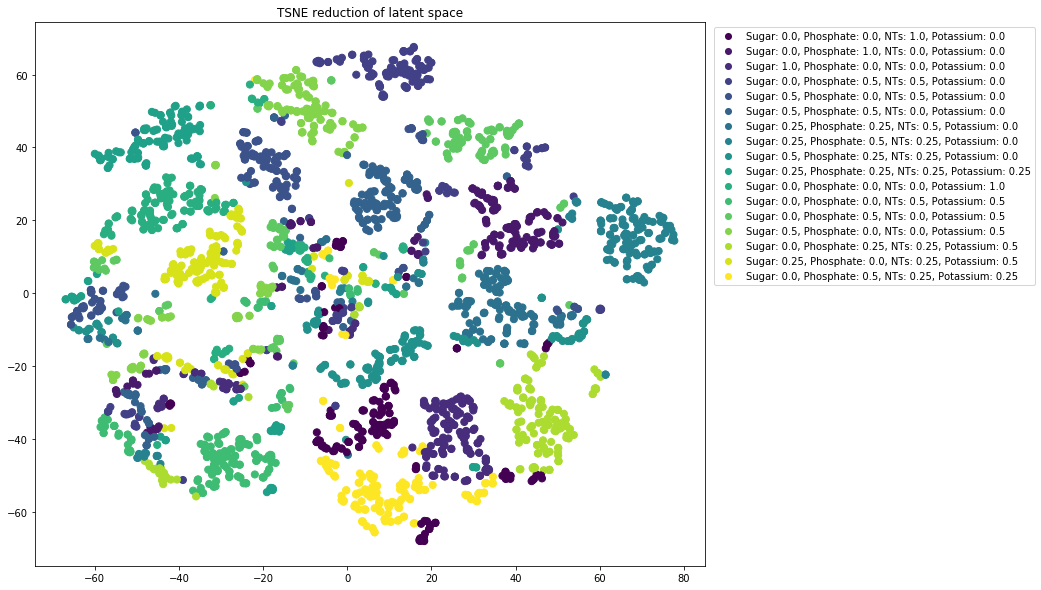
\includegraphics{figs/TSNE_hand_latent10.png}
\caption{We show that we can reconstruct each individual model from the latent space.}
\end{center}
\label{fig:ingest}
\end{figure}

We can see that the \gls{vae} is able to cluster the models reasonably well based on the experimental conditions.
This is a good sign because it means the \gls{vae} is able to distinguish between the fluxes of each model when we vary the experimental conditions.
Additionally, similar experimental conditions appear to be closer to each other.
For example, we can see the yellow dots at the bottom are near to two clusters of purple dots.
All three of the experimental conditions have no additional sugar and raised phosphate levels.
This implies that the latent space of the \gls{vae} can not only distinguish between experimental conditions but the distance in the latent space has biological meaning.

\section{Validation}
We also validated that our \gls{vae} was performing as intended.
We can examine a few aspects of our reconstructed fluxes to ensure that the results we are seeing are not simply due to chance.
Figure \ref{fig:fig:recon_stds} plots the standard deviations of each of the reactions for our test dataset as well as our reconstructed dataset.
We can see that the reconstructed dataset maintains a very similar shape to our original dataset, while also reducing the standard deviation of fluxes with each reaction.
Although we did not investigate this further, this implies that the \gls{vae} could also be used to de-noise our dataset.

\begin{figure}[t!]
\begin{center}
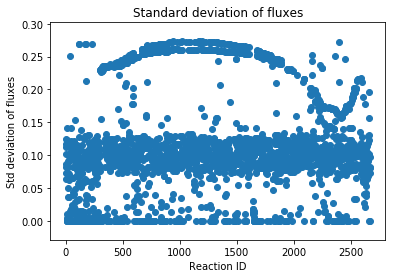
\includegraphics{figs/Reconstructed_stds.png}
\caption{Reconstructed fluxes reduce the amount of noise while also maintaining the shape}
\end{center}
\label{fig:recon_stds}
\end{figure}

Another key point we investigated was whether or not the correlations we produce are spurious.
We wanted to ensure that our \gls{vae} is not creating correlations out of thin air just to reduce its loss function.
Figure \ref{fig:noise} shows what happens when we add noise to our experimental data.
First, we generate a dataset with fluxes that are highly correlated to our experimental data.
This is represented by the green line. 
We can then run those fluxes through our \gls{vae} and check the correlation.
The blue line shows that this improves the correlation of our fluxes because of our loss function.
Next, we can add noise to the data by randomly drawing from a normal distribution and adding it to the flux for each reaction.
The dots show that as we add increasing amounts of noise to the data, the correlation goes to about 0.
This means that the \gls{vae} is not simply artificially creating a correlation but is learning something about the underlying data.

\begin{figure}[t!]
\begin{center}
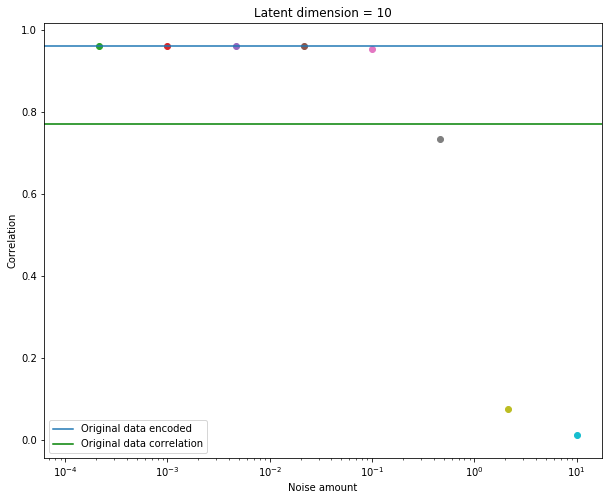
\includegraphics{figs/Noise_add.png}
\caption{Adding noise to the data reduces the correlation from our \gls{vae}}
\end{center}
\label{fig:noise}
\end{figure}

\section{Transfer learning}

TODO

%\section{Biological insights}